\documentclass[conference]{IEEEtran}

\usepackage{graphicx}

%\usepackage{biblatex}
\usepackage[backend=biber, style=authoryear]{biblatex}
\bibliography{bibliography}

\usepackage{enumitem,amssymb}
\newlist{todolist}{itemize}{1}
\setlist[todolist]{label=$\square$}

\usepackage{pgfplots}
\pgfplotsset{compat=1.8}
\usepgfplotslibrary{statistics}

\usepackage{CJKutf8}
\usepackage{float}

\begin{document}

% paper title
% Titles are generally capitalized except for words such as a, an, and, as,
% at, but, by, for, in, nor, of, on, or, the, to and up, which are usually
% not capitalized unless they are the first or last word of the title.
% Linebreaks \\ can be used within to get better formatting as desired.
% Do not put math or special symbols in the title.

% \title{Communication Technologies for \\Children in Rural China, \\Left Behind from Migrant-Working Parents \vspace{0.5cm}}
\title{Communication Technologies for \\Left-Behind Children in Rural China \vspace{0.5cm}}

% author names and affiliations
% use a multiple column layout for up to three different
% affiliations
\author{\IEEEauthorblockN{Matteo Yann Feo}
\IEEEauthorblockA{Master of Computer Science\\
Swiss Federal Institute of Technology, EPFL\\
Lausanne, Switzerland\\
Email: matteo.feo@epfl.ch}
\and
\IEEEauthorblockN{Simone Aron Sanso}
\IEEEauthorblockA{Master of Micro Engineering\\
Swiss Federal Institute of Technology, EPFL\\
Lausanne, Switzerland\\
Email: simone.sanso@epfl.ch}}

% conference papers do not typically use \thanks and this command
% is locked out in conference mode. If really needed, such as for
% the acknowledgment of grants, issue a \IEEEoverridecommandlockouts
% after \documentclass

% make the title area
\maketitle

%to force the numbering of the pages
\thispagestyle{plain}
\pagestyle{plain}

% As a general rule, do not put math, special symbols or citations in the abstract
\begin{abstract}
Starting from a literature review focusing on the effects of distant parenting on left-behind children in rural China, it has been shown that increased remittances (i.e. sending of money) allowed an enhancement of physical health and academic performance. However, mental health was found to be seriously affected by the lack of parental care, thus increasing the likelihood of depressions during the children's growth. A comparative analysis has been then realized, comparing three different scenarios of distant parenting: the first one covered the hospitalization of children, the second incarcerated parents and the third transnational parents, out-migrating for the same reason of the Chinese context. All three scenarios revealed the importance and the pros of communication technologies in distant parenting situations. To validate our assumptions, a survey has been forwarded towards parents and children having lived at distance during a continuous period of time, because of activities organized for the children (boy-scouting, summer camps and intercultural exchange programs). Both parents and children demonstrated to rate as essential the importance of communication between parents and children at distance. With even stronger and more sensitive settings than those joyful ones presented here, we anticipate how even more crucial the communication technologies might be rated by families of left-behind children. During an interview with an expert in Chinese anthropology and urban sociology, this hypothesis has been ascertained. Envisioning further investigations on the Chinese field, an interview protocol has been implemented and can be used to validate or refute our hypothesis, by questioning parents of left-behind children. Furthermore, the interview protocol provides a useful tool to analyze more in-depth the psychological effects of parents in this situation.

\end{abstract}

% no keywords

\section*{List of abbreviation}

% IDK, maybe ? -> Possiamo chiedere a Marc se ci sta

\begin{table}[ht]
    \centering
    \begin{tabular}{lll}
        CRC     &&      Convention on the Rights of the Child \\
        LBC     &&      Left-Behind Children \\
                &&              \\
        XYZ     &&      Lorem ipsum ... \\
        ABC     &&      Lorem ipsum...                     
    \end{tabular}
\end{table}

\section{Related work}
\label{related-work}

A large amount of studies have been conducted about the reality of left-behind children, on different localities around the world. These studies have been focusing on different impacts of parental migration, from the children's perspective. Interestingly, this phenomenon is not only restricted to China (\cite{song2009health}; \cite{he2012depression}; \cite{guo2017effect}; \cite{fan2010emotional}; \cite{bai2017effect}), but also frequently appears in Mexico (\cite{sawyer2016money}; \cite{kanaiaupuni2000reframing}; \cite{hildebrandt2005effects}; \cite{fernandez1998fathers}; \cite{dreby2007children}), Latin America (\cite{mundial2006development}; \cite{acosta2007impact}; \cite{anton2010impact}), Romania (\cite{botezat2014impact}), Philippines (\cite{yang2008international}; \cite{cortes2015feminization}; \cite{arguillas2010impact}) and Thailand (\cite{jampaklay2006parental}). In this section, specific terms used throughout the research will be defined. Then, related work will be reviewed, about the impact of parental migration on physical health, academic performance and mental health of left-behind children. 

\subsection{Definitions and terminology}

According to the United Nations (\cite{united1998recommendations}), the commonly accepted definition of 'migrant' is "any person who changes his or her country of usual residence". A more precise classification can be introduced with time and space constraints (\cite{rossi2008impact}). The process is then defined as "permanent", "long-term" (at least 12 months) or "seasonal", with either an internal or an international migration. Purposes of recreation, holiday, visits to friends, business, medical treatment, or religious pilgrimages are, although, not considered as migration processes (\cite{united1998recommendations}). Two scenarios of parental migration can appear. Either the parents migrate with their children, or they leave them behind (\cite{rossi2008impact}). Another possible result of parental migration is related to the issue of foster children. Although they share the same loss of parental care, the complete interruption of communication with both parents determines a completely different case that cannot be discussed nor compared with the two previously mentioned scenarios (\cite{pilon2003foster}). The commonly accepted definition of LBCs (\textit{left-behind children}) refers to children who stay at home when one or both parents relocate elsewhere, to join the labor force, for at least six months (\cite{lu2011left}). In the Chinese context, parental migration is considered to be seasonal and internal, since migrants move from rural to industrialized regions, spending yearly around 11 months away and returning home during the \textit{Spring Festival}. The formal definition of 'children', given in the CRC (\textit{Convention on the Rights of the Child}), Article 1 drafted by \textcite{unicef1989convention}, states that "individuals below the age of 18" form the children population. However, other conventions to define 'children' can be found. The 0-15 age range is the most adopted one, in accordance with the research context, due to medical (women fertility) and labor (legal working age) reasons.

\subsection{Impact on LBCs' physical health}

The study of \textcite{guo2017effect} reveals that the "overall effect" of parental migration on children's health is uncertain. 

Several researches found positive effects of parental migration on children's health (\cite{mundial2006development}; \cite{acosta2007impact}; \cite{anton2010impact}; \cite{stillman2012impact}) and have mainly attributed them for the increased incomes of the family. Remittances helped reducing childbirth mortality (\cite{hildebrandt2005effects}), increasing birth weight and decreasing the number of underweight newborns (\cite{frank2002other}). Children are better nourished and can take advantage from an eased access to health services (\cite{nobles2006contribution}). As a consequence, higher incomes enable the children to better manage chronic health problems through medication (\cite{case2002economic}).

Other researches raised negative effects of parental migration (\cite{amato1999nonresident}; \cite{kanaiaupuni2000reframing}; \cite{fernandez1998fathers}), mainly due to the reduction of parental care. \textcite{song2009health} found that LBCs started to overuse health services. A possible cause of this behaviour is the attempt to replace the lacking parental care by medical services. Another intriguing fact from this study is that the access to health services depended on whom the children were left with. Statistically, maternal migration had a negative effect on children's health. This result confirms several studies showing that maternal presence is essential for the development of a child (\cite{cortes2015feminization}; \cite{jampaklay2006parental}; \cite{macours2010seasonal}; \cite{thomas1994like}). With paternal migration, longer time and distance of migration positively affected children's health, again as a consequence of increased remittances. Children's health status revealed to be also affected by socio-economic factors, dependant on the household (\cite{behrman1996impact}). One reason why poor parents do not out-migrate could be the need of initial capital to cover emigration costs, for transportation and accommodation reasons. Lastly, health impact of parental migration has been shown to be independent to the child's age and gender (\cite{guo2017effect}). 

\subsection{Impact on LBCs' academic performance}

The study of \textcite{bai2017effect} rejected the hypothesis that parental migration deteriorated the academic performance of children. Additionally, they found that when one parent or both out-migrated, the academic performance of LBCs was even significantly improving, compared to the rest of the students. Increased incomes can therefore bring a larger impact than the reduction of parental care. Rising incomes might provide several benefits for LBCs, like a better nutrition, improved access to educational materials and less housework responsibilities. An analysis about the heterogeneity of the impact, among children of different households, showed that the positive effect of parental migration was even larger for students initially poorly performing at school. An explanation for LBCs' academic improvements is the availability of additional materials, which might have led them overcoming educational barriers that limited their performances. For instance, better nourished students see their academic performance rising (\cite{luo2012nutrition}). Remittances could also be invested in tutoring and other additional learning materials like books, computers and learning software. The positive impact of parental migration has been found to become larger when the out-migrating parent had a poor level of education. If the parent has a high level of education, a trade off between parental tutoring and migrant remittances appears. Therefore, depending on the out-migrating parent's background, the impact on the academic performance can significantly differ among LBCs (\cite{sawyer2016money}). 

\subsection{Impact on LBCs' mental health}

According to the study of \textcite{he2012depression}, LBCs were at greater risk to develop depression, compared to the other students. The work confirmed a previous study from \textcite{fan2010emotional}, conducted on the same topic. The emotional disturbances and higher risks of depression are more evident in specific age-ranges. During the early adolescence, changes in sexual cognition and social development occur, leading to determinant consequences for the overall maturity process. Without parental care, psychological problems occurring in the late childhood and adolescence can introduce direct repercussions on LBCs' mental health, increasing the indicators of adult depression risks  (\cite{kosterman2010assessment}).

The results presented in the Chinese context were further confirmed by another study, deriving evidences from Romania (\cite{botezat2014impact}), where the migration fluxes end towards more occidental European regions. The study illustrates substantial increases in depression, as well as higher propensity to be bullied during the childhood, more particularly in rural areas. These research insights match previous results from the literature on the mental health of left-behind children (\cite{gibson2011happens}; \cite{dreby2007children}; \cite{mazzucato2011transnational}). Children left alone to take care of themselves, living in an environment without any adult supervision, result in even larger risks of depression (\cite{lahaie2009work}).

\textcite{ren2016consequences} realized a more philosophical research about the possibility of wrongly perceiving causes of depression with Chinese LBCs. The research compared the difference of family "arrangements", or emotional bonds between parents and children, in China and other countries where the phenomenon of parental migration frequently occurs (i.e. Nicaragua, Philippines, Mexico). They concluded that, in the Chinese context, these family arrangements have "little impact on the emotional well-being of children". For this reason, researches about LBCs in the specific context of China should be considered a singularity of its own, due to the impressive number of internal migrants, incomparable to any other country. From the Chinese point of view, since the situation of leaving children behind became more common in rural areas (\cite{hao2006discussion}), non-Chinese researchers shall be cautious about their belief of understanding the local social context in China.





\section{Related work}
\label{related-work}

A large amount of studies have been conducted about the reality of left-behind children, on different localities around the world. These studies have been focusing on different impacts of parental migration, from the children's perspective. Interestingly, this phenomenon is not only restricted to China (\cite{song2009health}; \cite{he2012depression}; \cite{guo2017effect}; \cite{fan2010emotional}; \cite{bai2017effect}), but also frequently appears in Mexico (\cite{sawyer2016money}; \cite{kanaiaupuni2000reframing}; \cite{hildebrandt2005effects}; \cite{fernandez1998fathers}; \cite{dreby2007children}), Latin America (\cite{mundial2006development}; \cite{acosta2007impact}; \cite{anton2010impact}), Romania (\cite{botezat2014impact}), Philippines (\cite{yang2008international}; \cite{cortes2015feminization}; \cite{arguillas2010impact}) and Thailand (\cite{jampaklay2006parental}). In this section, specific terms used throughout the research will be defined. Then, related work will be reviewed, about the impact of parental migration on physical health, academic performance and mental health of left-behind children. 

\subsection{Definitions and terminology}

According to the United Nations (\cite{united1998recommendations}), the commonly accepted definition of 'migrant' is "any person who changes his or her country of usual residence". A more precise classification can be introduced with time and space constraints (\cite{rossi2008impact}). The process is then defined as "permanent", "long-term" (at least 12 months) or "seasonal", with either an internal or an international migration. Purposes of recreation, holiday, visits to friends, business, medical treatment, or religious pilgrimages are, although, not considered as migration processes (\cite{united1998recommendations}). Two scenarios of parental migration can appear. Either the parents migrate with their children, or they leave them behind (\cite{rossi2008impact}). Another possible result of parental migration is related to the issue of foster children. Although they share the same loss of parental care, the complete interruption of communication with both parents determines a completely different case that cannot be discussed nor compared with the two previously mentioned scenarios (\cite{pilon2003foster}). The commonly accepted definition of LBCs (\textit{left-behind children}) refers to children who stay at home when one or both parents relocate elsewhere, to join the labor force, for at least six months (\cite{lu2011left}). In the Chinese context, parental migration is considered to be seasonal and internal, since migrants move from rural to industrialized regions, spending yearly around 11 months away and returning home during the \textit{Spring Festival}. The formal definition of 'children', given in the CRC (\textit{Convention on the Rights of the Child}), Article 1 drafted by \textcite{unicef1989convention}, states that "individuals below the age of 18" form the children population. However, other conventions to define 'children' can be found. The 0-15 age range is the most adopted one, in accordance with the research context, due to medical (women fertility) and labor (legal working age) reasons.

\subsection{Impact on LBCs' physical health}

The study of \textcite{guo2017effect} reveals that the "overall effect" of parental migration on children's health is uncertain. 

Several researches found positive effects of parental migration on children's health (\cite{mundial2006development}; \cite{acosta2007impact}; \cite{anton2010impact}; \cite{stillman2012impact}) and have mainly attributed them for the increased incomes of the family. Remittances helped reducing childbirth mortality (\cite{hildebrandt2005effects}), increasing birth weight and decreasing the number of underweight newborns (\cite{frank2002other}). Children are better nourished and can take advantage from an eased access to health services (\cite{nobles2006contribution}). As a consequence, higher incomes enable the children to better manage chronic health problems through medication (\cite{case2002economic}).

Other researches raised negative effects of parental migration (\cite{amato1999nonresident}; \cite{kanaiaupuni2000reframing}; \cite{fernandez1998fathers}), mainly due to the reduction of parental care. \textcite{song2009health} found that LBCs started to overuse health services. A possible cause of this behaviour is the attempt to replace the lacking parental care by medical services. Another intriguing fact from this study is that the access to health services depended on whom the children were left with. Statistically, maternal migration had a negative effect on children's health. This result confirms several studies showing that maternal presence is essential for the development of a child (\cite{cortes2015feminization}; \cite{jampaklay2006parental}; \cite{macours2010seasonal}; \cite{thomas1994like}). With paternal migration, longer time and distance of migration positively affected children's health, again as a consequence of increased remittances. Children's health status revealed to be also affected by socio-economic factors, dependant on the household (\cite{behrman1996impact}). One reason why poor parents do not out-migrate could be the need of initial capital to cover emigration costs, for transportation and accommodation reasons. Lastly, health impact of parental migration has been shown to be independent to the child's age and gender (\cite{guo2017effect}). 

\subsection{Impact on LBCs' academic performance}

The study of \textcite{bai2017effect} rejected the hypothesis that parental migration deteriorated the academic performance of children. Additionally, they found that when one parent or both out-migrated, the academic performance of LBCs was even significantly improving, compared to the rest of the students. Increased incomes can therefore bring a larger impact than the reduction of parental care. Rising incomes might provide several benefits for LBCs, like a better nutrition, improved access to educational materials and less housework responsibilities. An analysis about the heterogeneity of the impact, among children of different households, showed that the positive effect of parental migration was even larger for students initially poorly performing at school. An explanation for LBCs' academic improvements is the availability of additional materials, which might have led them overcoming educational barriers that limited their performances. For instance, better nourished students see their academic performance rising (\cite{luo2012nutrition}). Remittances could also be invested in tutoring and other additional learning materials like books, computers and learning software. The positive impact of parental migration has been found to become larger when the out-migrating parent had a poor level of education. If the parent has a high level of education, a trade off between parental tutoring and migrant remittances appears. Therefore, depending on the out-migrating parent's background, the impact on the academic performance can significantly differ among LBCs (\cite{sawyer2016money}). 

\subsection{Impact on LBCs' mental health}

According to the study of \textcite{he2012depression}, LBCs were at greater risk to develop depression, compared to the other students. The work confirmed a previous study from \textcite{fan2010emotional}, conducted on the same topic. The emotional disturbances and higher risks of depression are more evident in specific age-ranges. During the early adolescence, changes in sexual cognition and social development occur, leading to determinant consequences for the overall maturity process. Without parental care, psychological problems occurring in the late childhood and adolescence can introduce direct repercussions on LBCs' mental health, increasing the indicators of adult depression risks  (\cite{kosterman2010assessment}).

The results presented in the Chinese context were further confirmed by another study, deriving evidences from Romania (\cite{botezat2014impact}), where the migration fluxes end towards more occidental European regions. The study illustrates substantial increases in depression, as well as higher propensity to be bullied during the childhood, more particularly in rural areas. These research insights match previous results from the literature on the mental health of left-behind children (\cite{gibson2011happens}; \cite{dreby2007children}; \cite{mazzucato2011transnational}). Children left alone to take care of themselves, living in an environment without any adult supervision, result in even larger risks of depression (\cite{lahaie2009work}).

\textcite{ren2016consequences} realized a more philosophical research about the possibility of wrongly perceiving causes of depression with Chinese LBCs. The research compared the difference of family "arrangements", or emotional bonds between parents and children, in China and other countries where the phenomenon of parental migration frequently occurs (i.e. Nicaragua, Philippines, Mexico). They concluded that, in the Chinese context, these family arrangements have "little impact on the emotional well-being of children". For this reason, researches about LBCs in the specific context of China should be considered a singularity of its own, due to the impressive number of internal migrants, incomparable to any other country. From the Chinese point of view, since the situation of leaving children behind became more common in rural areas (\cite{hao2006discussion}), non-Chinese researchers shall be cautious about their belief of understanding the local social context in China.





\section{Related work}
\label{related-work}

A large amount of studies have been conducted about the reality of left-behind children, on different localities around the world. These studies have been focusing on different impacts of parental migration, from the children's perspective. Interestingly, this phenomenon is not only restricted to China (\cite{song2009health}; \cite{he2012depression}; \cite{guo2017effect}; \cite{fan2010emotional}; \cite{bai2017effect}), but also frequently appears in Mexico (\cite{sawyer2016money}; \cite{kanaiaupuni2000reframing}; \cite{hildebrandt2005effects}; \cite{fernandez1998fathers}; \cite{dreby2007children}), Latin America (\cite{mundial2006development}; \cite{acosta2007impact}; \cite{anton2010impact}), Romania (\cite{botezat2014impact}), Philippines (\cite{yang2008international}; \cite{cortes2015feminization}; \cite{arguillas2010impact}) and Thailand (\cite{jampaklay2006parental}). In this section, specific terms used throughout the research will be defined. Then, related work will be reviewed, about the impact of parental migration on physical health, academic performance and mental health of left-behind children. 

\subsection{Definitions and terminology}

According to the United Nations (\cite{united1998recommendations}), the commonly accepted definition of 'migrant' is "any person who changes his or her country of usual residence". A more precise classification can be introduced with time and space constraints (\cite{rossi2008impact}). The process is then defined as "permanent", "long-term" (at least 12 months) or "seasonal", with either an internal or an international migration. Purposes of recreation, holiday, visits to friends, business, medical treatment, or religious pilgrimages are, although, not considered as migration processes (\cite{united1998recommendations}). Two scenarios of parental migration can appear. Either the parents migrate with their children, or they leave them behind (\cite{rossi2008impact}). Another possible result of parental migration is related to the issue of foster children. Although they share the same loss of parental care, the complete interruption of communication with both parents determines a completely different case that cannot be discussed nor compared with the two previously mentioned scenarios (\cite{pilon2003foster}). The commonly accepted definition of LBCs (\textit{left-behind children}) refers to children who stay at home when one or both parents relocate elsewhere, to join the labor force, for at least six months (\cite{lu2011left}). In the Chinese context, parental migration is considered to be seasonal and internal, since migrants move from rural to industrialized regions, spending yearly around 11 months away and returning home during the \textit{Spring Festival}. The formal definition of 'children', given in the CRC (\textit{Convention on the Rights of the Child}), Article 1 drafted by \textcite{unicef1989convention}, states that "individuals below the age of 18" form the children population. However, other conventions to define 'children' can be found. The 0-15 age range is the most adopted one, in accordance with the research context, due to medical (women fertility) and labor (legal working age) reasons.

\subsection{Impact on LBCs' physical health}

The study of \textcite{guo2017effect} reveals that the "overall effect" of parental migration on children's health is uncertain. 

Several researches found positive effects of parental migration on children's health (\cite{mundial2006development}; \cite{acosta2007impact}; \cite{anton2010impact}; \cite{stillman2012impact}) and have mainly attributed them for the increased incomes of the family. Remittances helped reducing childbirth mortality (\cite{hildebrandt2005effects}), increasing birth weight and decreasing the number of underweight newborns (\cite{frank2002other}). Children are better nourished and can take advantage from an eased access to health services (\cite{nobles2006contribution}). As a consequence, higher incomes enable the children to better manage chronic health problems through medication (\cite{case2002economic}).

Other researches raised negative effects of parental migration (\cite{amato1999nonresident}; \cite{kanaiaupuni2000reframing}; \cite{fernandez1998fathers}), mainly due to the reduction of parental care. \textcite{song2009health} found that LBCs started to overuse health services. A possible cause of this behaviour is the attempt to replace the lacking parental care by medical services. Another intriguing fact from this study is that the access to health services depended on whom the children were left with. Statistically, maternal migration had a negative effect on children's health. This result confirms several studies showing that maternal presence is essential for the development of a child (\cite{cortes2015feminization}; \cite{jampaklay2006parental}; \cite{macours2010seasonal}; \cite{thomas1994like}). With paternal migration, longer time and distance of migration positively affected children's health, again as a consequence of increased remittances. Children's health status revealed to be also affected by socio-economic factors, dependant on the household (\cite{behrman1996impact}). One reason why poor parents do not out-migrate could be the need of initial capital to cover emigration costs, for transportation and accommodation reasons. Lastly, health impact of parental migration has been shown to be independent to the child's age and gender (\cite{guo2017effect}). 

\subsection{Impact on LBCs' academic performance}

The study of \textcite{bai2017effect} rejected the hypothesis that parental migration deteriorated the academic performance of children. Additionally, they found that when one parent or both out-migrated, the academic performance of LBCs was even significantly improving, compared to the rest of the students. Increased incomes can therefore bring a larger impact than the reduction of parental care. Rising incomes might provide several benefits for LBCs, like a better nutrition, improved access to educational materials and less housework responsibilities. An analysis about the heterogeneity of the impact, among children of different households, showed that the positive effect of parental migration was even larger for students initially poorly performing at school. An explanation for LBCs' academic improvements is the availability of additional materials, which might have led them overcoming educational barriers that limited their performances. For instance, better nourished students see their academic performance rising (\cite{luo2012nutrition}). Remittances could also be invested in tutoring and other additional learning materials like books, computers and learning software. The positive impact of parental migration has been found to become larger when the out-migrating parent had a poor level of education. If the parent has a high level of education, a trade off between parental tutoring and migrant remittances appears. Therefore, depending on the out-migrating parent's background, the impact on the academic performance can significantly differ among LBCs (\cite{sawyer2016money}). 

\subsection{Impact on LBCs' mental health}

According to the study of \textcite{he2012depression}, LBCs were at greater risk to develop depression, compared to the other students. The work confirmed a previous study from \textcite{fan2010emotional}, conducted on the same topic. The emotional disturbances and higher risks of depression are more evident in specific age-ranges. During the early adolescence, changes in sexual cognition and social development occur, leading to determinant consequences for the overall maturity process. Without parental care, psychological problems occurring in the late childhood and adolescence can introduce direct repercussions on LBCs' mental health, increasing the indicators of adult depression risks  (\cite{kosterman2010assessment}).

The results presented in the Chinese context were further confirmed by another study, deriving evidences from Romania (\cite{botezat2014impact}), where the migration fluxes end towards more occidental European regions. The study illustrates substantial increases in depression, as well as higher propensity to be bullied during the childhood, more particularly in rural areas. These research insights match previous results from the literature on the mental health of left-behind children (\cite{gibson2011happens}; \cite{dreby2007children}; \cite{mazzucato2011transnational}). Children left alone to take care of themselves, living in an environment without any adult supervision, result in even larger risks of depression (\cite{lahaie2009work}).

\textcite{ren2016consequences} realized a more philosophical research about the possibility of wrongly perceiving causes of depression with Chinese LBCs. The research compared the difference of family "arrangements", or emotional bonds between parents and children, in China and other countries where the phenomenon of parental migration frequently occurs (i.e. Nicaragua, Philippines, Mexico). They concluded that, in the Chinese context, these family arrangements have "little impact on the emotional well-being of children". For this reason, researches about LBCs in the specific context of China should be considered a singularity of its own, due to the impressive number of internal migrants, incomparable to any other country. From the Chinese point of view, since the situation of leaving children behind became more common in rural areas (\cite{hao2006discussion}), non-Chinese researchers shall be cautious about their belief of understanding the local social context in China.





\section{Related work}
\label{related-work}

A large amount of studies have been conducted about the reality of left-behind children, on different localities around the world. These studies have been focusing on different impacts of parental migration, from the children's perspective. Interestingly, this phenomenon is not only restricted to China (\cite{song2009health}; \cite{he2012depression}; \cite{guo2017effect}; \cite{fan2010emotional}; \cite{bai2017effect}), but also frequently appears in Mexico (\cite{sawyer2016money}; \cite{kanaiaupuni2000reframing}; \cite{hildebrandt2005effects}; \cite{fernandez1998fathers}; \cite{dreby2007children}), Latin America (\cite{mundial2006development}; \cite{acosta2007impact}; \cite{anton2010impact}), Romania (\cite{botezat2014impact}), Philippines (\cite{yang2008international}; \cite{cortes2015feminization}; \cite{arguillas2010impact}) and Thailand (\cite{jampaklay2006parental}). In this section, specific terms used throughout the research will be defined. Then, related work will be reviewed, about the impact of parental migration on physical health, academic performance and mental health of left-behind children. 

\subsection{Definitions and terminology}

According to the United Nations (\cite{united1998recommendations}), the commonly accepted definition of 'migrant' is "any person who changes his or her country of usual residence". A more precise classification can be introduced with time and space constraints (\cite{rossi2008impact}). The process is then defined as "permanent", "long-term" (at least 12 months) or "seasonal", with either an internal or an international migration. Purposes of recreation, holiday, visits to friends, business, medical treatment, or religious pilgrimages are, although, not considered as migration processes (\cite{united1998recommendations}). Two scenarios of parental migration can appear. Either the parents migrate with their children, or they leave them behind (\cite{rossi2008impact}). Another possible result of parental migration is related to the issue of foster children. Although they share the same loss of parental care, the complete interruption of communication with both parents determines a completely different case that cannot be discussed nor compared with the two previously mentioned scenarios (\cite{pilon2003foster}). The commonly accepted definition of LBCs (\textit{left-behind children}) refers to children who stay at home when one or both parents relocate elsewhere, to join the labor force, for at least six months (\cite{lu2011left}). In the Chinese context, parental migration is considered to be seasonal and internal, since migrants move from rural to industrialized regions, spending yearly around 11 months away and returning home during the \textit{Spring Festival}. The formal definition of 'children', given in the CRC (\textit{Convention on the Rights of the Child}), Article 1 drafted by \textcite{unicef1989convention}, states that "individuals below the age of 18" form the children population. However, other conventions to define 'children' can be found. The 0-15 age range is the most adopted one, in accordance with the research context, due to medical (women fertility) and labor (legal working age) reasons.

\subsection{Impact on LBCs' physical health}

The study of \textcite{guo2017effect} reveals that the "overall effect" of parental migration on children's health is uncertain. 

Several researches found positive effects of parental migration on children's health (\cite{mundial2006development}; \cite{acosta2007impact}; \cite{anton2010impact}; \cite{stillman2012impact}) and have mainly attributed them for the increased incomes of the family. Remittances helped reducing childbirth mortality (\cite{hildebrandt2005effects}), increasing birth weight and decreasing the number of underweight newborns (\cite{frank2002other}). Children are better nourished and can take advantage from an eased access to health services (\cite{nobles2006contribution}). As a consequence, higher incomes enable the children to better manage chronic health problems through medication (\cite{case2002economic}).

Other researches raised negative effects of parental migration (\cite{amato1999nonresident}; \cite{kanaiaupuni2000reframing}; \cite{fernandez1998fathers}), mainly due to the reduction of parental care. \textcite{song2009health} found that LBCs started to overuse health services. A possible cause of this behaviour is the attempt to replace the lacking parental care by medical services. Another intriguing fact from this study is that the access to health services depended on whom the children were left with. Statistically, maternal migration had a negative effect on children's health. This result confirms several studies showing that maternal presence is essential for the development of a child (\cite{cortes2015feminization}; \cite{jampaklay2006parental}; \cite{macours2010seasonal}; \cite{thomas1994like}). With paternal migration, longer time and distance of migration positively affected children's health, again as a consequence of increased remittances. Children's health status revealed to be also affected by socio-economic factors, dependant on the household (\cite{behrman1996impact}). One reason why poor parents do not out-migrate could be the need of initial capital to cover emigration costs, for transportation and accommodation reasons. Lastly, health impact of parental migration has been shown to be independent to the child's age and gender (\cite{guo2017effect}). 

\subsection{Impact on LBCs' academic performance}

The study of \textcite{bai2017effect} rejected the hypothesis that parental migration deteriorated the academic performance of children. Additionally, they found that when one parent or both out-migrated, the academic performance of LBCs was even significantly improving, compared to the rest of the students. Increased incomes can therefore bring a larger impact than the reduction of parental care. Rising incomes might provide several benefits for LBCs, like a better nutrition, improved access to educational materials and less housework responsibilities. An analysis about the heterogeneity of the impact, among children of different households, showed that the positive effect of parental migration was even larger for students initially poorly performing at school. An explanation for LBCs' academic improvements is the availability of additional materials, which might have led them overcoming educational barriers that limited their performances. For instance, better nourished students see their academic performance rising (\cite{luo2012nutrition}). Remittances could also be invested in tutoring and other additional learning materials like books, computers and learning software. The positive impact of parental migration has been found to become larger when the out-migrating parent had a poor level of education. If the parent has a high level of education, a trade off between parental tutoring and migrant remittances appears. Therefore, depending on the out-migrating parent's background, the impact on the academic performance can significantly differ among LBCs (\cite{sawyer2016money}). 

\subsection{Impact on LBCs' mental health}

According to the study of \textcite{he2012depression}, LBCs were at greater risk to develop depression, compared to the other students. The work confirmed a previous study from \textcite{fan2010emotional}, conducted on the same topic. The emotional disturbances and higher risks of depression are more evident in specific age-ranges. During the early adolescence, changes in sexual cognition and social development occur, leading to determinant consequences for the overall maturity process. Without parental care, psychological problems occurring in the late childhood and adolescence can introduce direct repercussions on LBCs' mental health, increasing the indicators of adult depression risks  (\cite{kosterman2010assessment}).

The results presented in the Chinese context were further confirmed by another study, deriving evidences from Romania (\cite{botezat2014impact}), where the migration fluxes end towards more occidental European regions. The study illustrates substantial increases in depression, as well as higher propensity to be bullied during the childhood, more particularly in rural areas. These research insights match previous results from the literature on the mental health of left-behind children (\cite{gibson2011happens}; \cite{dreby2007children}; \cite{mazzucato2011transnational}). Children left alone to take care of themselves, living in an environment without any adult supervision, result in even larger risks of depression (\cite{lahaie2009work}).

\textcite{ren2016consequences} realized a more philosophical research about the possibility of wrongly perceiving causes of depression with Chinese LBCs. The research compared the difference of family "arrangements", or emotional bonds between parents and children, in China and other countries where the phenomenon of parental migration frequently occurs (i.e. Nicaragua, Philippines, Mexico). They concluded that, in the Chinese context, these family arrangements have "little impact on the emotional well-being of children". For this reason, researches about LBCs in the specific context of China should be considered a singularity of its own, due to the impressive number of internal migrants, incomparable to any other country. From the Chinese point of view, since the situation of leaving children behind became more common in rural areas (\cite{hao2006discussion}), non-Chinese researchers shall be cautious about their belief of understanding the local social context in China.





\section{Related work}
\label{related-work}

A large amount of studies have been conducted about the reality of left-behind children, on different localities around the world. These studies have been focusing on different impacts of parental migration, from the children's perspective. Interestingly, this phenomenon is not only restricted to China (\cite{song2009health}; \cite{he2012depression}; \cite{guo2017effect}; \cite{fan2010emotional}; \cite{bai2017effect}), but also frequently appears in Mexico (\cite{sawyer2016money}; \cite{kanaiaupuni2000reframing}; \cite{hildebrandt2005effects}; \cite{fernandez1998fathers}; \cite{dreby2007children}), Latin America (\cite{mundial2006development}; \cite{acosta2007impact}; \cite{anton2010impact}), Romania (\cite{botezat2014impact}), Philippines (\cite{yang2008international}; \cite{cortes2015feminization}; \cite{arguillas2010impact}) and Thailand (\cite{jampaklay2006parental}). In this section, specific terms used throughout the research will be defined. Then, related work will be reviewed, about the impact of parental migration on physical health, academic performance and mental health of left-behind children. 

\subsection{Definitions and terminology}

According to the United Nations (\cite{united1998recommendations}), the commonly accepted definition of 'migrant' is "any person who changes his or her country of usual residence". A more precise classification can be introduced with time and space constraints (\cite{rossi2008impact}). The process is then defined as "permanent", "long-term" (at least 12 months) or "seasonal", with either an internal or an international migration. Purposes of recreation, holiday, visits to friends, business, medical treatment, or religious pilgrimages are, although, not considered as migration processes (\cite{united1998recommendations}). Two scenarios of parental migration can appear. Either the parents migrate with their children, or they leave them behind (\cite{rossi2008impact}). Another possible result of parental migration is related to the issue of foster children. Although they share the same loss of parental care, the complete interruption of communication with both parents determines a completely different case that cannot be discussed nor compared with the two previously mentioned scenarios (\cite{pilon2003foster}). The commonly accepted definition of LBCs (\textit{left-behind children}) refers to children who stay at home when one or both parents relocate elsewhere, to join the labor force, for at least six months (\cite{lu2011left}). In the Chinese context, parental migration is considered to be seasonal and internal, since migrants move from rural to industrialized regions, spending yearly around 11 months away and returning home during the \textit{Spring Festival}. The formal definition of 'children', given in the CRC (\textit{Convention on the Rights of the Child}), Article 1 drafted by \textcite{unicef1989convention}, states that "individuals below the age of 18" form the children population. However, other conventions to define 'children' can be found. The 0-15 age range is the most adopted one, in accordance with the research context, due to medical (women fertility) and labor (legal working age) reasons.

\subsection{Impact on LBCs' physical health}

The study of \textcite{guo2017effect} reveals that the "overall effect" of parental migration on children's health is uncertain. 

Several researches found positive effects of parental migration on children's health (\cite{mundial2006development}; \cite{acosta2007impact}; \cite{anton2010impact}; \cite{stillman2012impact}) and have mainly attributed them for the increased incomes of the family. Remittances helped reducing childbirth mortality (\cite{hildebrandt2005effects}), increasing birth weight and decreasing the number of underweight newborns (\cite{frank2002other}). Children are better nourished and can take advantage from an eased access to health services (\cite{nobles2006contribution}). As a consequence, higher incomes enable the children to better manage chronic health problems through medication (\cite{case2002economic}).

Other researches raised negative effects of parental migration (\cite{amato1999nonresident}; \cite{kanaiaupuni2000reframing}; \cite{fernandez1998fathers}), mainly due to the reduction of parental care. \textcite{song2009health} found that LBCs started to overuse health services. A possible cause of this behaviour is the attempt to replace the lacking parental care by medical services. Another intriguing fact from this study is that the access to health services depended on whom the children were left with. Statistically, maternal migration had a negative effect on children's health. This result confirms several studies showing that maternal presence is essential for the development of a child (\cite{cortes2015feminization}; \cite{jampaklay2006parental}; \cite{macours2010seasonal}; \cite{thomas1994like}). With paternal migration, longer time and distance of migration positively affected children's health, again as a consequence of increased remittances. Children's health status revealed to be also affected by socio-economic factors, dependant on the household (\cite{behrman1996impact}). One reason why poor parents do not out-migrate could be the need of initial capital to cover emigration costs, for transportation and accommodation reasons. Lastly, health impact of parental migration has been shown to be independent to the child's age and gender (\cite{guo2017effect}). 

\subsection{Impact on LBCs' academic performance}

The study of \textcite{bai2017effect} rejected the hypothesis that parental migration deteriorated the academic performance of children. Additionally, they found that when one parent or both out-migrated, the academic performance of LBCs was even significantly improving, compared to the rest of the students. Increased incomes can therefore bring a larger impact than the reduction of parental care. Rising incomes might provide several benefits for LBCs, like a better nutrition, improved access to educational materials and less housework responsibilities. An analysis about the heterogeneity of the impact, among children of different households, showed that the positive effect of parental migration was even larger for students initially poorly performing at school. An explanation for LBCs' academic improvements is the availability of additional materials, which might have led them overcoming educational barriers that limited their performances. For instance, better nourished students see their academic performance rising (\cite{luo2012nutrition}). Remittances could also be invested in tutoring and other additional learning materials like books, computers and learning software. The positive impact of parental migration has been found to become larger when the out-migrating parent had a poor level of education. If the parent has a high level of education, a trade off between parental tutoring and migrant remittances appears. Therefore, depending on the out-migrating parent's background, the impact on the academic performance can significantly differ among LBCs (\cite{sawyer2016money}). 

\subsection{Impact on LBCs' mental health}

According to the study of \textcite{he2012depression}, LBCs were at greater risk to develop depression, compared to the other students. The work confirmed a previous study from \textcite{fan2010emotional}, conducted on the same topic. The emotional disturbances and higher risks of depression are more evident in specific age-ranges. During the early adolescence, changes in sexual cognition and social development occur, leading to determinant consequences for the overall maturity process. Without parental care, psychological problems occurring in the late childhood and adolescence can introduce direct repercussions on LBCs' mental health, increasing the indicators of adult depression risks  (\cite{kosterman2010assessment}).

The results presented in the Chinese context were further confirmed by another study, deriving evidences from Romania (\cite{botezat2014impact}), where the migration fluxes end towards more occidental European regions. The study illustrates substantial increases in depression, as well as higher propensity to be bullied during the childhood, more particularly in rural areas. These research insights match previous results from the literature on the mental health of left-behind children (\cite{gibson2011happens}; \cite{dreby2007children}; \cite{mazzucato2011transnational}). Children left alone to take care of themselves, living in an environment without any adult supervision, result in even larger risks of depression (\cite{lahaie2009work}).

\textcite{ren2016consequences} realized a more philosophical research about the possibility of wrongly perceiving causes of depression with Chinese LBCs. The research compared the difference of family "arrangements", or emotional bonds between parents and children, in China and other countries where the phenomenon of parental migration frequently occurs (i.e. Nicaragua, Philippines, Mexico). They concluded that, in the Chinese context, these family arrangements have "little impact on the emotional well-being of children". For this reason, researches about LBCs in the specific context of China should be considered a singularity of its own, due to the impressive number of internal migrants, incomparable to any other country. From the Chinese point of view, since the situation of leaving children behind became more common in rural areas (\cite{hao2006discussion}), non-Chinese researchers shall be cautious about their belief of understanding the local social context in China.





\section{Related work}
\label{related-work}

A large amount of studies have been conducted about the reality of left-behind children, on different localities around the world. These studies have been focusing on different impacts of parental migration, from the children's perspective. Interestingly, this phenomenon is not only restricted to China (\cite{song2009health}; \cite{he2012depression}; \cite{guo2017effect}; \cite{fan2010emotional}; \cite{bai2017effect}), but also frequently appears in Mexico (\cite{sawyer2016money}; \cite{kanaiaupuni2000reframing}; \cite{hildebrandt2005effects}; \cite{fernandez1998fathers}; \cite{dreby2007children}), Latin America (\cite{mundial2006development}; \cite{acosta2007impact}; \cite{anton2010impact}), Romania (\cite{botezat2014impact}), Philippines (\cite{yang2008international}; \cite{cortes2015feminization}; \cite{arguillas2010impact}) and Thailand (\cite{jampaklay2006parental}). In this section, specific terms used throughout the research will be defined. Then, related work will be reviewed, about the impact of parental migration on physical health, academic performance and mental health of left-behind children. 

\subsection{Definitions and terminology}

According to the United Nations (\cite{united1998recommendations}), the commonly accepted definition of 'migrant' is "any person who changes his or her country of usual residence". A more precise classification can be introduced with time and space constraints (\cite{rossi2008impact}). The process is then defined as "permanent", "long-term" (at least 12 months) or "seasonal", with either an internal or an international migration. Purposes of recreation, holiday, visits to friends, business, medical treatment, or religious pilgrimages are, although, not considered as migration processes (\cite{united1998recommendations}). Two scenarios of parental migration can appear. Either the parents migrate with their children, or they leave them behind (\cite{rossi2008impact}). Another possible result of parental migration is related to the issue of foster children. Although they share the same loss of parental care, the complete interruption of communication with both parents determines a completely different case that cannot be discussed nor compared with the two previously mentioned scenarios (\cite{pilon2003foster}). The commonly accepted definition of LBCs (\textit{left-behind children}) refers to children who stay at home when one or both parents relocate elsewhere, to join the labor force, for at least six months (\cite{lu2011left}). In the Chinese context, parental migration is considered to be seasonal and internal, since migrants move from rural to industrialized regions, spending yearly around 11 months away and returning home during the \textit{Spring Festival}. The formal definition of 'children', given in the CRC (\textit{Convention on the Rights of the Child}), Article 1 drafted by \textcite{unicef1989convention}, states that "individuals below the age of 18" form the children population. However, other conventions to define 'children' can be found. The 0-15 age range is the most adopted one, in accordance with the research context, due to medical (women fertility) and labor (legal working age) reasons.

\subsection{Impact on LBCs' physical health}

The study of \textcite{guo2017effect} reveals that the "overall effect" of parental migration on children's health is uncertain. 

Several researches found positive effects of parental migration on children's health (\cite{mundial2006development}; \cite{acosta2007impact}; \cite{anton2010impact}; \cite{stillman2012impact}) and have mainly attributed them for the increased incomes of the family. Remittances helped reducing childbirth mortality (\cite{hildebrandt2005effects}), increasing birth weight and decreasing the number of underweight newborns (\cite{frank2002other}). Children are better nourished and can take advantage from an eased access to health services (\cite{nobles2006contribution}). As a consequence, higher incomes enable the children to better manage chronic health problems through medication (\cite{case2002economic}).

Other researches raised negative effects of parental migration (\cite{amato1999nonresident}; \cite{kanaiaupuni2000reframing}; \cite{fernandez1998fathers}), mainly due to the reduction of parental care. \textcite{song2009health} found that LBCs started to overuse health services. A possible cause of this behaviour is the attempt to replace the lacking parental care by medical services. Another intriguing fact from this study is that the access to health services depended on whom the children were left with. Statistically, maternal migration had a negative effect on children's health. This result confirms several studies showing that maternal presence is essential for the development of a child (\cite{cortes2015feminization}; \cite{jampaklay2006parental}; \cite{macours2010seasonal}; \cite{thomas1994like}). With paternal migration, longer time and distance of migration positively affected children's health, again as a consequence of increased remittances. Children's health status revealed to be also affected by socio-economic factors, dependant on the household (\cite{behrman1996impact}). One reason why poor parents do not out-migrate could be the need of initial capital to cover emigration costs, for transportation and accommodation reasons. Lastly, health impact of parental migration has been shown to be independent to the child's age and gender (\cite{guo2017effect}). 

\subsection{Impact on LBCs' academic performance}

The study of \textcite{bai2017effect} rejected the hypothesis that parental migration deteriorated the academic performance of children. Additionally, they found that when one parent or both out-migrated, the academic performance of LBCs was even significantly improving, compared to the rest of the students. Increased incomes can therefore bring a larger impact than the reduction of parental care. Rising incomes might provide several benefits for LBCs, like a better nutrition, improved access to educational materials and less housework responsibilities. An analysis about the heterogeneity of the impact, among children of different households, showed that the positive effect of parental migration was even larger for students initially poorly performing at school. An explanation for LBCs' academic improvements is the availability of additional materials, which might have led them overcoming educational barriers that limited their performances. For instance, better nourished students see their academic performance rising (\cite{luo2012nutrition}). Remittances could also be invested in tutoring and other additional learning materials like books, computers and learning software. The positive impact of parental migration has been found to become larger when the out-migrating parent had a poor level of education. If the parent has a high level of education, a trade off between parental tutoring and migrant remittances appears. Therefore, depending on the out-migrating parent's background, the impact on the academic performance can significantly differ among LBCs (\cite{sawyer2016money}). 

\subsection{Impact on LBCs' mental health}

According to the study of \textcite{he2012depression}, LBCs were at greater risk to develop depression, compared to the other students. The work confirmed a previous study from \textcite{fan2010emotional}, conducted on the same topic. The emotional disturbances and higher risks of depression are more evident in specific age-ranges. During the early adolescence, changes in sexual cognition and social development occur, leading to determinant consequences for the overall maturity process. Without parental care, psychological problems occurring in the late childhood and adolescence can introduce direct repercussions on LBCs' mental health, increasing the indicators of adult depression risks  (\cite{kosterman2010assessment}).

The results presented in the Chinese context were further confirmed by another study, deriving evidences from Romania (\cite{botezat2014impact}), where the migration fluxes end towards more occidental European regions. The study illustrates substantial increases in depression, as well as higher propensity to be bullied during the childhood, more particularly in rural areas. These research insights match previous results from the literature on the mental health of left-behind children (\cite{gibson2011happens}; \cite{dreby2007children}; \cite{mazzucato2011transnational}). Children left alone to take care of themselves, living in an environment without any adult supervision, result in even larger risks of depression (\cite{lahaie2009work}).

\textcite{ren2016consequences} realized a more philosophical research about the possibility of wrongly perceiving causes of depression with Chinese LBCs. The research compared the difference of family "arrangements", or emotional bonds between parents and children, in China and other countries where the phenomenon of parental migration frequently occurs (i.e. Nicaragua, Philippines, Mexico). They concluded that, in the Chinese context, these family arrangements have "little impact on the emotional well-being of children". For this reason, researches about LBCs in the specific context of China should be considered a singularity of its own, due to the impressive number of internal migrants, incomparable to any other country. From the Chinese point of view, since the situation of leaving children behind became more common in rural areas (\cite{hao2006discussion}), non-Chinese researchers shall be cautious about their belief of understanding the local social context in China.





% conference papers do not normally have an appendix

% use section* for acknowledgment
\section*{Acknowledgment}
We would like to thank the contacted associations (listed in the appendix \ref{appendix:contacts_list}) that helped us forwarding the survey about the importance of communication. We are also grateful to the 116 persons who spent a few minutes answering the survey. Finally, last but by no means least, a very special gratitude goes out to Mr. Laperrouza,  Ms. Graezer Bideau, Ms. Preissmann and our peer-reviewers who assisted us during this research. It has been a fantastic opportunity to work with experts and have insights from different fields on the question of LBC in rural China. 

\printbibliography

\vfill
\listoffigures

\listoftables

\clearpage
% Appendix of the Report
\appendix

In the following appendix are presented the questions of the survey (... a list of figures and tables) to the reader.

\subsection{Questions of the survey}
\label{appendix:survey_questions}
In this section is shown how the participants were questioned towards the survey. Only the questions in English will be shown here, skipping the French translations.

\medskip \textit{Form about communication technologies :} \\
Realizing a research project about social sciences within EPFL University (Lausanne), we would like to understand the importance of communication between parents and children, when they are at a distance during a continuous period of time.

\vspace{4pt}
1. In what language would like to answer this form?

2. To contextualize, we seek either :

- parents of a child having spent a period of time away from the household,

- children, teenagers and young adults having spent a period of time away from their family.

After having read the description above, do you qualify yourself as a parent or a child?

\vspace{4pt}
\noindent - If "parent" was selected question 2: 

3.a. Are you the mother or the father?

4.a. Have you already been separated from your child for at least 3 days? (Exchange semester abroad, holidays, summer camp, boy-scout, etc.)

5.a. If there were more than one experience of distance parenting, please consider the earliest one of them through the rest of the form (when you were the youngest). What is the reason why your child was distant from you? 

6.a. For how long have you been distant from your child?

7.a. How old was your child at that time?

8.a. What is your child's gender?

9.a. How often did you use a communication technology with your distant child? (Text messages, phone calls, video chat, etc.)

10.a. What kind of information did you seek from communicating with your distant child?

11.a. How would you define the importance of being able to communicate with your distant child?

\vspace{4pt}
\noindent - If "child" was selected question 2: 

3.b. Have you already been separated from your family for at least 3 days? (Exchange semester abroad, holidays, summer camp, boy-scout, etc.)

3.b. If there were more than one experience of separation from your family, please consider the earliest one of them through the rest of the form (when you were the youngest). What is the reason why you were distant from your family? 

4.b. For how long have you been away?

5.b. How old were you at that time?

6.b. What is your gender?

7.b. How often did you use a communication technology with your family? (Text messages, phone calls, video chat, etc.)

8.b. What kind of information did you seek from communicating with your family?

9.b. How would you define the importance of being able to communicate with your family?


\subsection{Additional plots of the results}
\label{appendix:additional-plots}

The following plots have been computed for the analysis of the data collected via the survey on distant-parenting. This appendix contains a set of plots that didn't need particular attention during the discussion, but can still be source of investigation.

\begin{figure}[h!]
    \centering
    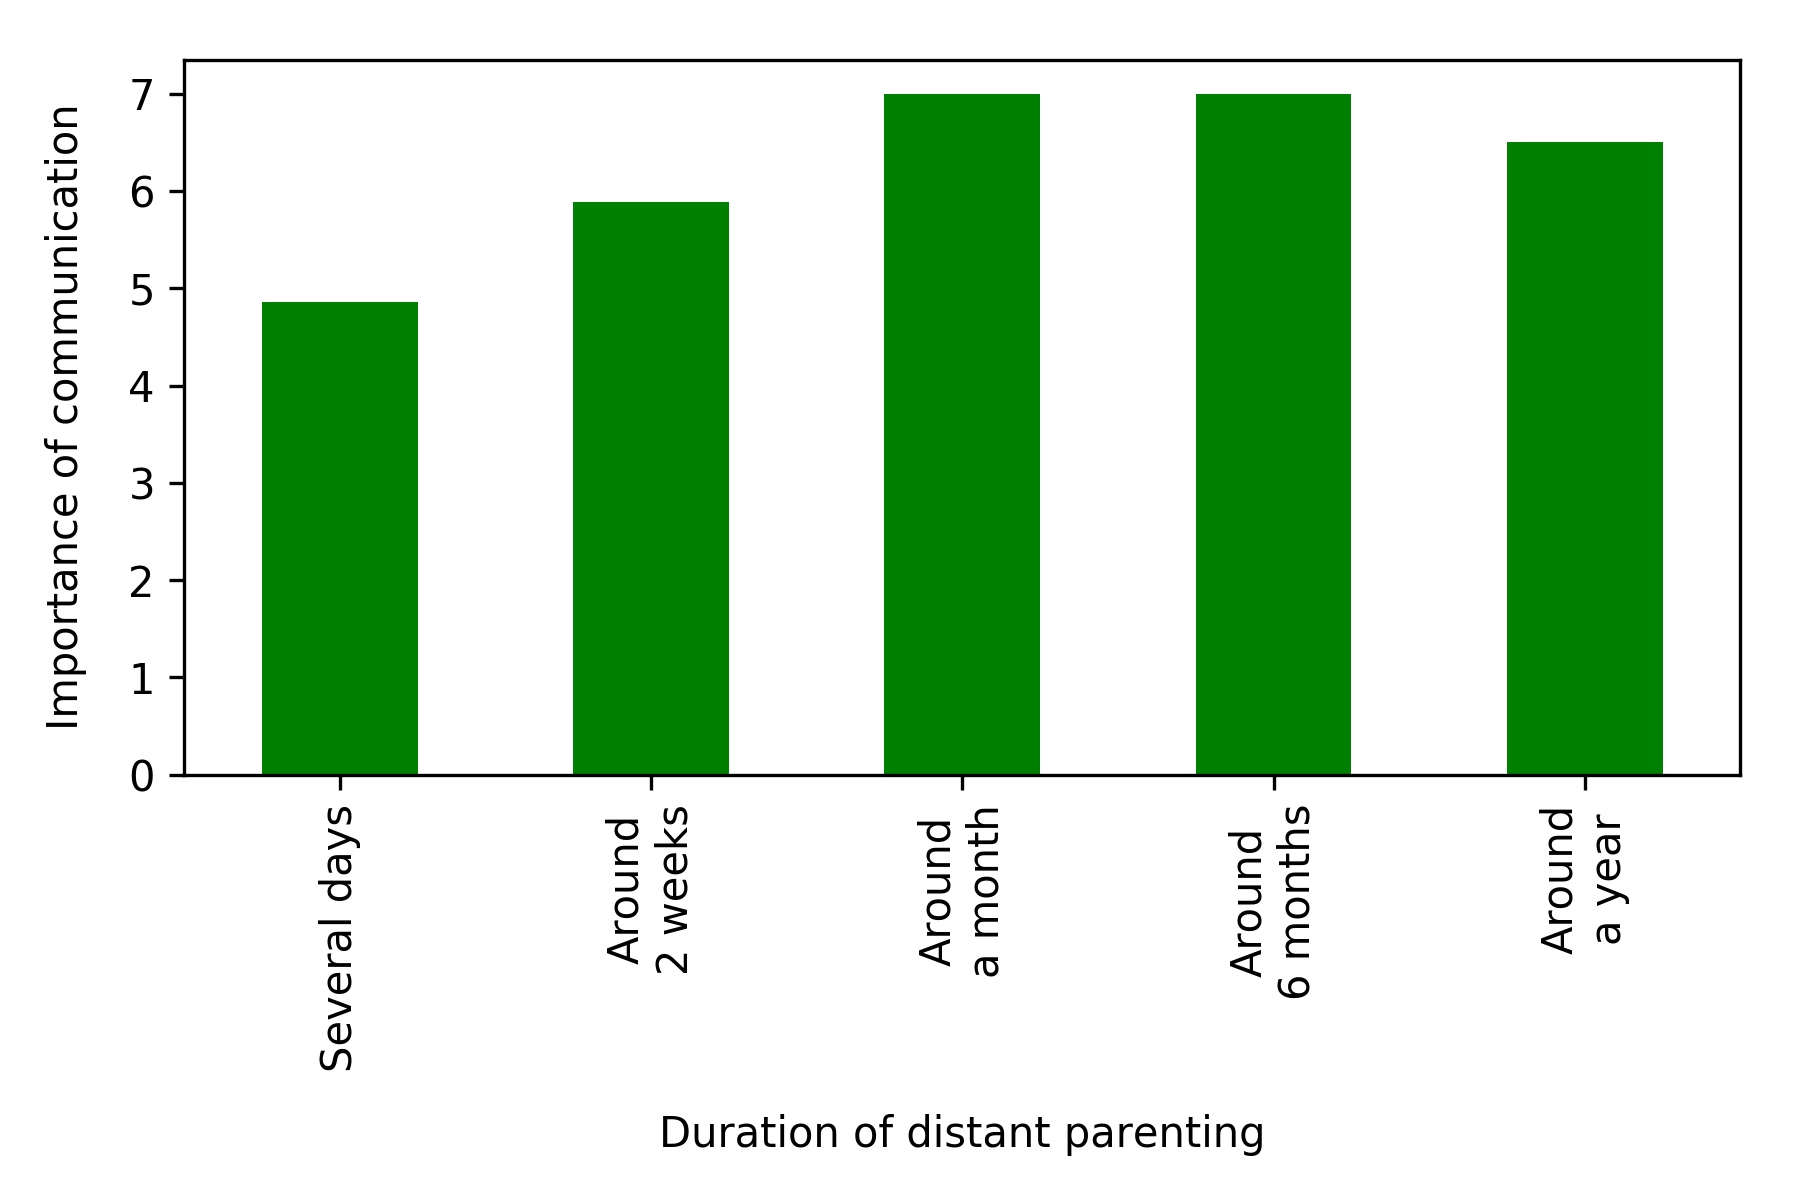
\includegraphics[scale=0.58]{plots/plot_5.png}
    \caption{Importance of communication from the parent point according to duration of distant-parenting experience}
    \label{fig:plot_5}
\end{figure}

\begin{figure}[h!]
    \centering
    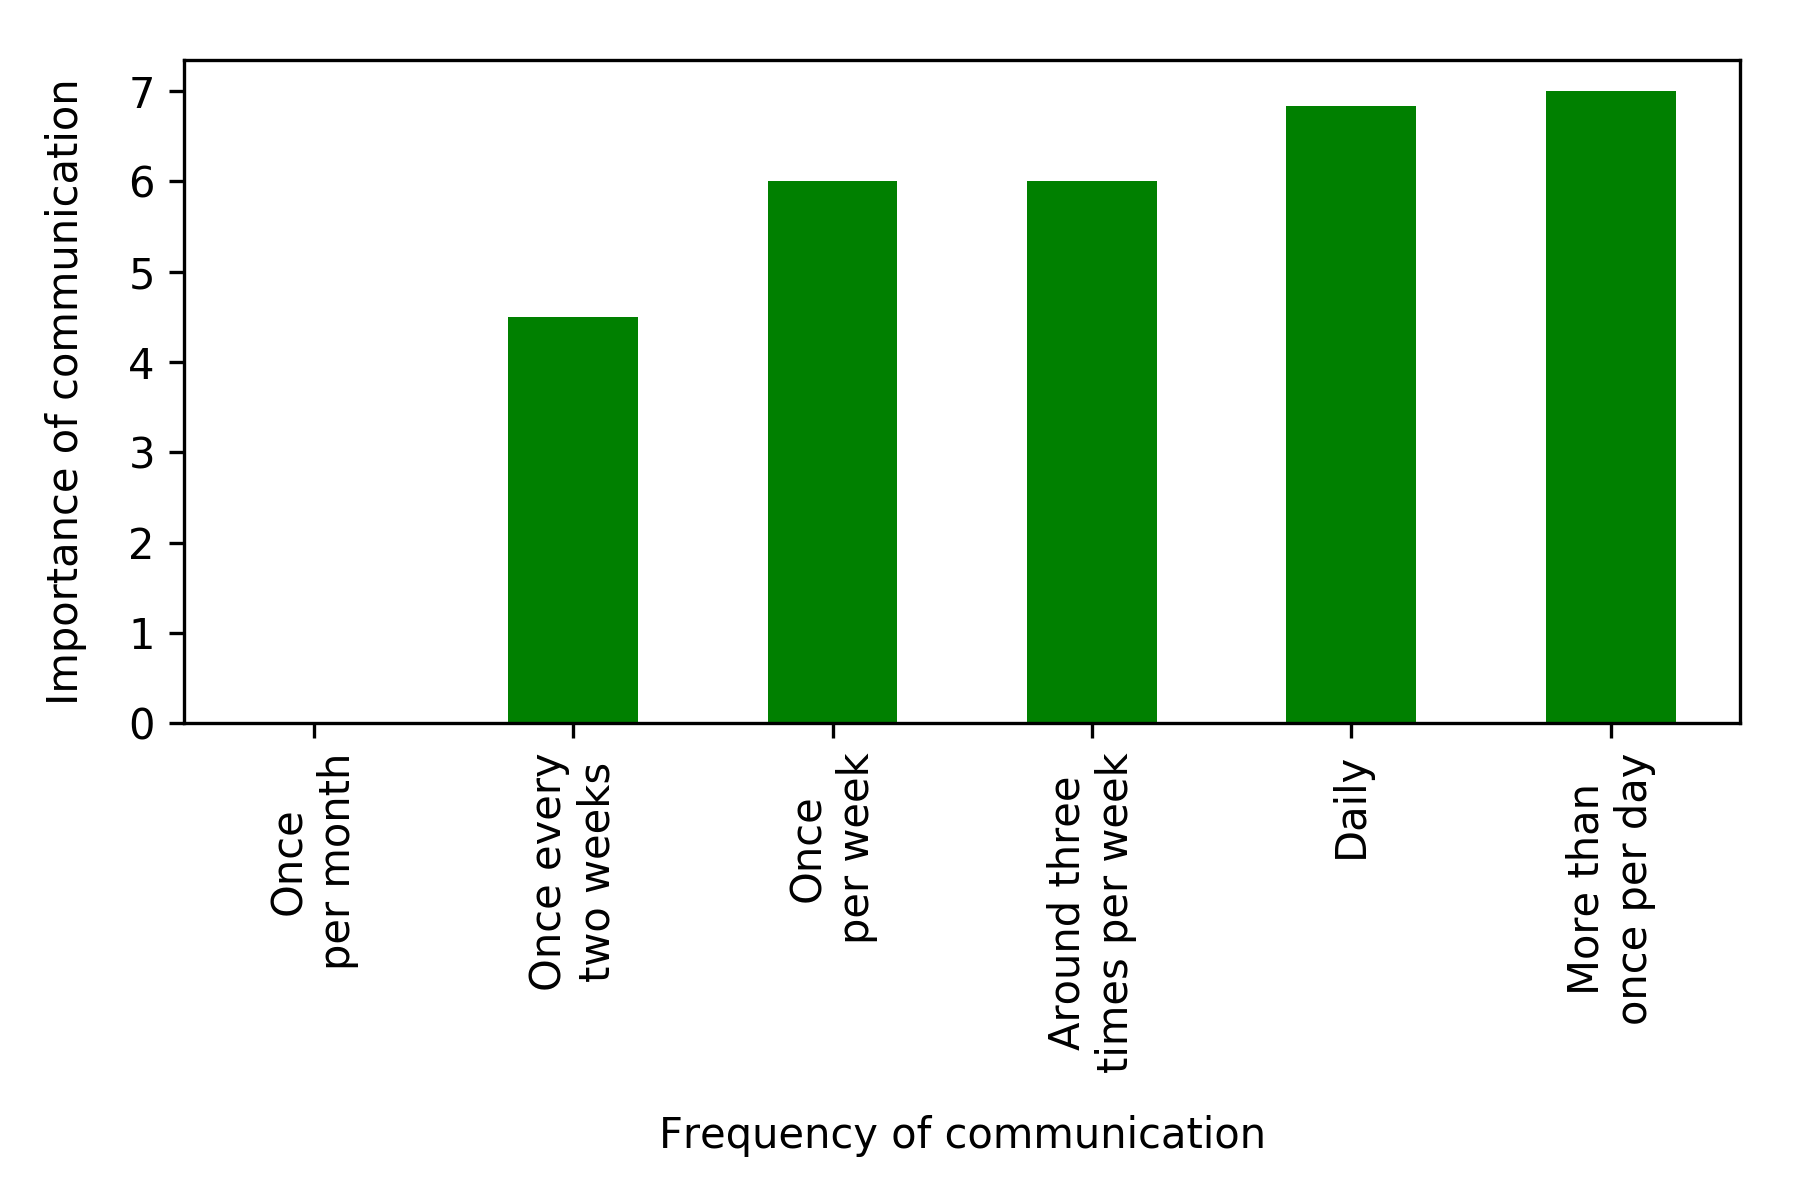
\includegraphics[scale=0.58]{plots/plot_8.png}
    \caption{Importance of communication from the parent point according to frequency of communication during distant-parenting experience}
    \label{fig:plot_8}
\end{figure}


\subsection{Interview protocol}
\label{appendix:interview_protocol}

The following interview protocol has been prepared for the research on “Communication Technologies for Left-Behind Children in Rural China”, in the scope of the “Global perspectives, local realities” SHS course. To continue our research on the Chinese field, by interviewing parents of left behind children, our assumptions could be tested and eventually further analyzed.

\vspace{4pt}
Please, fill in the missing informations as follows before starting the interview session:

Author: Matteo Yann Feo \& Simone Sanso

Session length: 40 minutes 

Participant Name: \hfill \_\_\_\_\_\_\_\_\_\_\_\_\_\_\_\_\_\_\_\_\_\_\_  $\leftarrow$ Fill in

Email: \hfill \_\_\_\_\_\_\_\_\_\_\_\_\_\_\_\_\_\_\_\_\_\_\_\_\_\_\_\_\_\_\_\_ $\leftarrow$ Fill in

Time/Date: \hfill \_\_\_\_\_\_\_\_\_\_\_\_\_\_\_\_\_\_\_\_\_\_\_\_\_\_\_\_ $\leftarrow$ Fill in

Location: \hfill \_\_\_\_\_\_\_\_\_\_\_\_\_\_\_\_\_\_\_\_\_\_\_\_\_\_\_\_\_ $\leftarrow$ Fill in

\vspace{6pt}
\subsubsection{Introduction \& Setup (5 mins)}

The session starts with a short introduction to what this interview is about, the context and the background for which it is being conducted. In the meantime, be sure that everything is setup correctly by double checking the following To-Do list:

\begin{todolist}
    \item Setup the recording tools and check if they work correctly.
    \item Prepare note-taking utilities, such as pen and paper.
    \item Verify the environment, being sure to have a relaxed location for the following 40 mins.
    \item In case a beverage is desired in the meantime, be sure to have it ready and available now.
    \item Be sure that your interviewed person has everything needed.
\end{todolist}

The introduction of the interview could be similar to the following one:

"Good morning and thank you for participating! I am Yann. I am studying at EPFL for a master degree in computer science. My main interest for this interview is to understand whether  a  technology  of  communication embedded in a smart toy could be helpful for parents distant from their children. During the interview, I will be having a conversation with you, asking questions that could help me to achieve my curiosity. In the meantime, my partner, will be assisting me by taking some notes. It is important to always remember that we are not evaluating you or your opinions in any way, there are no possible right and wrong answers that you could give. 
Here is how the session is going to proceed. Firstly, we'll break the ice by asking you a few general questions to know each other. We will record this interview, given your consent. We won't ever share this recording nor use it for anything else but pure support for this interview, so that I can go back and review things later to make sure we got everything right. Your name won't ever be linked to any result, so be relaxed and feel free to share your thoughts with us, without any troubles. Keep in mind that this is completely voluntary, the recording can be stopped whenever you want. Thus, if you don't like this idea, please let me know. 
How does all that sound to you? Do you have any questions at this point?"

\begin{todolist}
    \item Ask the interviewee to sign the written consent for recording purposes.
\end{todolist}

\vspace{2pt}
\subsubsection{Demographics \& Background (5 mins)}

This section will help us to create a background of the interviewee, while allowing him/her to start opening up to our questions. Use this session as a warming-up occasion to break the ice, while catching the first important features. Start to note down details on the interviewee, like gender, age, education level, marital status.

\begin{todolist}
    \item Tell us your name, and a little bit about yourself.
    \item Where do you come from?
    \item What is your occupation? Are you studying or working? In both cases, can you tell us something about it?
    \item Where are you currently living? Do you live with someone, or alone? 
\end{todolist}

\vspace{2pt}
\subsubsection{Main questions (20 mins)}

The following questions can be helpful to interpolate your impressions with the interviewee’s feelings and personal stories. Use them carefully as they might be intimidating for some people. Don’t forget to check for nonverbal behaviors, as they might be critical to have a complete idea of who you are interviewing, especially in this part. Note that the most important questions to be answered are marked with an asterisk (*).

\vspace{2pt}
(*) Pre-interview questions about their children :

\begin{todolist}
    \item How many children do you have?
    \item How old are they?
    \item What gender are they?
    \item Where do you they live?
    \item With who are they staying in your home village? (Lonely, with one of both parents, with grandparents or other relatives)
\end{todolist}

Main interview questions about the interviewed parent :

\begin{todolist}
    \item (*) How often and for how long do you come back home? 
    \item What is the main reason why you live far away from your children?
    \item How do you feel about this situation, not living with your children?
    \item Remember the last time you went back to your home village, how was the contact with your children? Was the meeting with your children as before you left them?
    \item During your childhood, have you ever experienced living far away from one of your parents? If yes, for how long? How did you live the situation? Could you tell us what was the main reason of your parent to out-migrate? How was the contact when meeting again with your parent? Could you communicate together, at that time, while being distant? (Check for non-verbal reactions while interviewee showcase personal experience)
    \item How common is your situation of distant parenting? Do you know any other persons in the same situation as you? How do they live it?
    \item (*) How would you define the importance of living with your children? In your case, is there a trade off between living with your children and having a job position? If yes, imagine that you could live in an ideal world, what would be the best solution? Would you rather work in your home village or be able to bring your children in town?
    \item (*) Do you own electronic devices? If yes, which ones? (Smartphone, computer, more…)
    \item (*) Do your children in your home village own electronic devices? If not, would they have the opportunity to use any? (Neighbourhood, school, etc.)
    \item (*) Do you use electronic devices to contact your children? If yes, how often? In general, are you calling your children when you have time? Or do they also get in touch with you, on their initiative?
    \item (*) From 0 to 7, how would you define the importance of communicating with your children? (0: insignificant, 4: neutral, 7: essential) (Check for non-verbal reactions while interviewee showcase personal experience)
\end{todolist}

\vspace{2pt}
\subsubsection{Interviewee's "show and tell" prototype (8 mins)}

This section is practical and allows us to showcase our project, related to the issue of distant parenting. In the context of CHIC (China Hardware Innovation Camp), a plush toy that encourages social interaction between parents and children, in a distant situation. It is a very resourceful moment, as it could bring additional and authentic feedback on a novel user scenario.

The explanation of the prototype could be similar to the following one:

"We have been working on this prototype. It is a plush toy that encourages social interaction, by having remotely turned on LEDs and sounds from a mobile application. Parents and children can therefore stay longer connected. Letting your children know when you think about them will help you stay 'toygether'\texttrademark."

Showcase the prototype and how it works with the mobile application.

\begin{todolist}
    \item What do you think about the idea?
    \item In your opinion, which are the positive and negative aspects?
    \item If you had the possibility to try this technology, would you be interested?
    \item What would you modify to improve it?
\end{todolist}

\vspace{2pt}
\subsubsection{Closing (2 mins)}

Thank the user at the end for participating to the session. Offer the possibility to ask any kind of question the interviewee might want to address you.  This is his/her time to wear the interviewer's shoes in your regards.

If the interviewee has no additional question, the interview is officially finished. Thank again your interviewee for the time and availability to participate to this session. Underline how useful his/her help has been for the project.
Turn off the recording tools only when you are completely sure that nothing will be added. It is important to not miss anything, so better have some extra recording to cut later.

Take some time to, directly after the end of the interview, write down some impressions you may have about the session. It is important to note down very early impressions about both verbal and physical languages, before they are forgotten. Those are the most authentic resources to get.




\subsection{List of contacts}
\label{appendix:contacts_list}
Below are listed all the contacts that have been reached, to spread as much as possible the survey.

\begin{itemize}
\item AFS programs for adolescents (15-18 years old): \\
Duration: 1 year \\
Kernstrasse 57, CH-8004 Zurich \\
Tel: +41 21 323 19 19 \\
Email: hello@afs.ch \\
https://www.afs.ch/fr/programmes-scolaires/ 

\vspace{4pt}
\item Canada-France exchange (16 years old): \\
Duration : 3 weeks \\
College of Jeanne d'Arc, 15 Rue du Chanoine Brun, 68100 Mulhouse, France \\
Tel: +33 3 89 45 36 31 \\
www.ejda.fr/ 

\vspace{4pt}
\item International exchange programs (14-18 years old): \\
Duration: 1 year \\
Rue Centrale 15, 1003 Lausanne \\
Tel: +41 800 822 811 \\
https://www.efswiss.ch/fr/highschool/ 

\vspace{4pt}
\item National observatory of the Erasmus + impact (1 year or 6 months): \\
Email: observatoire@agence-erasmus.fr \\
http://www.agence-erasmus.fr/page/observatoire/

\vspace{4pt}
\item Journal of international mobility:\\
Email: revue@agence-erasmus.fr \\
https://www.agence-erasmus.fr/page/JIM

\vspace{4pt}
\item Exchange program Brigitte Sauzay (14-17 years old): \\
Duration: 3 months in a host family in Germany and welcome 3 months in the family in France \\
https://www.ofaj.org/contact.html 

\vspace{4pt}
\item Internal exchanges and language stays in Switzerland (14-17 years old): \\
Duration: 1 year \\
College of Delémont, Avenue Station 7, 2800 Delémont \\
Tel: +41 32 421 00 70 \\
Email: info@coldel.org \\
http://www.college-delemont.ch/fr/Aide-aux-eleves/Echanges-et-sejours-linguistiques/Echanges-et-sejours-linguistiques.html \\
Cantonal manager of linguistic exchanges: \\
Patrice KAMBER, Pâquerettes 2, 2822 Courroux \\
- Prof: 032 435 65 92 / Private: 032 422 83 62 

\vspace{4pt}
\item Language Exchange and Mobility - DIP Geneva: \\
Catherine Fernandez Sonino: Head of Exchange \& Mobility DIP of the Cantonal Office for Language Exchange and Mobility \\
Chemin de l'Echo 5a, 1213 Onex \\
Email: catherine.fernandez@etat.ge.ch \\
Tel: +41 22 327 06 43, +41 79 175 56 46 \\
https://edu.ge.ch/site/elem/ 

\vspace{4pt}
\item Service of primary and secondary schools of Lausanne: \\
Place Chauderon 9, 5th floor, PO Box 5032, 1002 Lausanne \\
Tel: +41 21 315 64 11 - Fax: +41 21 315 60 04 \\
Email: seps@lausanne.ch \\
http://www.lausanne.ch/etablissements-scolaires/ 

\vspace{4pt}
\item Summer camp of Neuchatel:\\
Gisèle Nicaty \\
Quartier du Milieu 86, 2127 Les Bayards \\
Tel: +41 79 288 50 41, +41 32 866 17 29\\
Email: giroud.p-a@bluewin.ch\\
http://www.echanges-scolaires.com/index.php/fr/

\vspace{4pt}
\item Summer camp of the Grandes-Roches: \\
1348 le Brassus \\
Tel: +41 21 845 66 90 \\
Email: camps@asime.ch \\
http://www.grandesroches.ch/home 

\vspace{4pt}
\item Association of the Gros-de-Vaud Holiday Camp: \\
Mrs Florence Ethenoz \\
Chemin du Petit Record 60, 1040 Echallens \\
Tel: +41 21 881 10 76 \\
Email: info@colo-gros-de-vaud.ch \\
http://www.colo-gros-de-vaud.ch/clubdesk/www

\vspace{4pt}
\item Summer camp 4Fun: \\
Email: airfred@hotmail.com \\
http://4-fun.ch/ 

\vspace{4pt}
\item Summer camp CPV: \\
Swiss Village Street 14, PO Box 72, 1211 Geneva 8 \\
Tel: +41 22 809 49 79 \\
Email: info@camps.ch \\
http://www.camps.ch/fr/accueil 

\vspace{4pt}
\item Scouts of the Sacred Heart: \\
Jeanne Voruz \& Anne Thiébaud \\
Tel: +41 79 844 92 74 \& +41 79 284 50 38 \\
Email: cg@sacrescout.ch \\
http://www.sacrescout.ch/ 

\vspace{4pt}
\item Village Camps: \\
PO Box 1425, Rue de la Morache 14, 1260 Nyon 1 \\
Tel: +41 22 990 9400 \\
Email: camps@villagecamps.com \\
www.villagecamps.com

\vspace{4pt}
\item Alpadia Language Schools: \\
Grand-Rue 42, PO Box 1206, 1820 Montreux\\
Tel: +41 21 621 88 88\\
Email: info@alpadia.com\\
https://www.alpadia.com/fr/ 

\vspace{4pt}
\item Carol Panchaud Educom sàrl: \\
26 Route of Givrins, CH - 1276 Gingins\\
Tel: +41 22 776 69 15 \\
Email: carolpanchaud@educom.ch \\
http://educom.ch/fr

\vspace{4pt}
\item Caritas-Youth: \\
11, Jean-Violette Street, 1205 Geneva\\
Tel: +41 22 708 04 04\\
Email: info@caritas-jeunesse.ch\\
http://www.caritas-jeunesse.ch/

\vspace{4pt}
\item Holiday Camp St. Gervais: \\
CP 1337, 1211 Geneva 1\\
Tel: +41 78 896 71 84\\
Email: info@colonie-saint-gervais.ch\\
http://www.colonie-saint-gervais.ch/

\vspace{4pt}
\item Summer Camp of Ravoire - Camp Plein Soleil: \\
PO Box 87, CH-1920 Martigny 1\\
Email: info@camp-pleinsoleil.ch

\vspace{4pt}
\item Yverdon-les-Bains youth service and social cohesion: \\
Rue de Neuchâtel 2, 1400 Yverdon-les-Bains\\
Tel: +41 24 423 69 11\\
Email: vacances@yverdon-les-bains.ch\\
http://www.yverdon-les-bains.ch/prestations-deladministration/jeunesse-et-cohesion-sociale/enfanceetfamille/colonies-dete-et-dautomne/

\vspace{4pt}
\item fRilingue GmbH: \\
Stöckackerstrasse 93, 3018 Bern\\
Tel: +41 26 321 34 34 \\
Email: info@frilingue.com

\vspace{4pt}
\item Star Sports: \\
Path of Verger 2, PO Box 101, 1304 Cossonay-Ville\\
Tel: +41 79 356 44 61\\
Email: info@starsports.ch\\
http://www.starsports.ch/

\vspace{4pt}
\item Cap Loisirs Foundation: \\
34, Boulevard de Saint-Georges, 1205 Geneva\\
Tel: +41 22 731 86 00\\
Email: caploisirs@caploisirs.ch\\
http://www.caploisirs.ch/

\vspace{4pt}
\item SCE Holidays \& Events: \\
Rue de Lausanne 58, 1950 Sion\\
Tel: +41 79 693.33.64\\
Email: info@lescamps.ch\\
https://www.lescamps.ch/\\

\end{itemize}




\end{document}


